\documentclass[letterpaper,journal]{IEEEtran}
\IEEEoverridecommandlockouts
\let\proof\relax\let\endproof\relax
\usepackage{amsmath,amssymb,amsthm}
\usepackage{graphicx,booktabs,xcolor}
\usepackage{dblfloatfix}
\renewcommand{\topfraction}{0.9}\renewcommand{\dbltopfraction}{0.9}\renewcommand{\textfraction}{0.07}\renewcommand{\floatpagefraction}{0.8}\renewcommand{\dblfloatpagefraction}{0.8}
\usepackage[hidelinks]{hyperref}
\newtheorem{lemma}{Lemma}
\newtheorem{proposition}{Proposition}
\newtheorem{corollary}{Corollary}
\theoremstyle{remark}
\newtheorem{remark}{Remark}
\newcommand{\D}{\mathcal{D}}
\newcommand{\W}{\mathcal{W}}
\DeclareMathOperator*{\argmin}{arg\,min}
\DeclareMathOperator*{\argmax}{arg\,max}

\title{When Should Robots Hide Where They Wait?\\ Leakage-Aware Randomized Staging for\\ Capacity-Constrained Multi-Robot Response}
\author{Syed Muhammad Alam and Hamza Rafique%
\thanks{S. M. Alam is with the Robotics, Intelligent Systems and Control (RISC) Lab, King Abdullah University of Science and Technology (KAUST), Thuwal, Saudi Arabia (e-mail: syed.alam@kaust.edu.sa). H. Rafique is with the Center for Water Informatics \& Technology (WIT) and the Department of Electrical Engineering, Lahore University of Management Sciences (LUMS), Lahore 54792, Pakistan (e-mail: hamza.rafique@lums.edu.pk).}}
\markboth{IEEE Robotics and Automation Letters. Preprint Version. Submitted 2026}{Alam and Rafique: Leakage-Aware Randomized Robot Staging}

\begin{document}
\maketitle

\begin{abstract}
Security or inspection robots wait at a few staging docks and must answer a burst of simultaneous alarms placed by an adversary. Randomizing where they wait can help, but only to the extent that the adversary cannot see the realized staging. We model this as a zero-sum game: the planner commits to a distribution over dock configurations, the adversary observes the realized configuration with probability $q$, and the planner answers with a capacity-limited, all-or-nothing robot assignment over path-time reachability. We show that per-site marginal probabilities do not determine the value, so marginal-coverage security-game formulations do not apply; that the value is convex in $q$ with a threshold $q^\star$ beyond which randomization loses its strict worst-case advantage; that $q^\star$ is computable by one linear-fractional program; and that randomizing among equally robust configurations is free. In 540 exact games the benefit concentrates where reachability is sparse and capacity tight (cell means up to 14.9\%) and shrinks with more docks. In closed-loop simulation, optimized randomization beats the best fixed staging by 8.1\%, 5.8\% and 2.6\% at $q=0,0.25,0.5$, whereas uniform randomization loses 12--18\%. Sensitivity analyses show the benefit is specific to all-or-nothing restoration with reliable robots. Gazebo/Nav2 travel times match the model ($R^2=0.995$); in concurrent three-robot Nav2 runs the benefit holds only after reachability is verified with the navigation stack. A matrix-free exact solver handles $3.3\times10^{11}$ attack allocations in seconds.
\end{abstract}

\begin{IEEEkeywords}
Multi-robot systems, planning, scheduling and coordination, robot safety, game theory, security.
\end{IEEEkeywords}

\section{Introduction}
Mobile robots are increasingly deployed to patrol, inspect and respond inside warehouses, plants and campuses. Between incidents they wait at staging docks, and when alarms fire they are dispatched to the affected zones. Where they wait determines what they can reach in time. If the alarms are caused by a strategic adversary---an intruder triggering sensors to overload the fleet, or a saboteur disabling several subsystems at once---the adversary will load the zones the fleet is least able to serve. A fixed staging plan is then a liability: once observed, it tells the adversary exactly where the gaps are.

Randomizing the staging configuration from shift to shift is the obvious remedy, and randomized defence is the core idea of security games~\cite{tambe2011,korzhyk2011}. Two features of robot response, however, are not captured by standard security-game models. First, a zone is restored only if \emph{all} of its alarms are served, and the robots at a dock are shared among zones, so the planner's payoff depends on which docks are open \emph{together}, not on how often each is open. Second, robots must physically relocate between shifts and staging is often partly visible: randomization is only as valuable as it is concealed. A planner therefore needs to know not just how to randomize, but whether randomizing is worth it given how much of the staging leaks.

This paper answers both questions for a capacity-constrained multi-robot response game. Our contributions are:
\begin{enumerate}
\item A \textbf{leakage-aware staging game}: the planner commits to a distribution over dock configurations; the adversary sees the realized configuration with probability $q$; the planner responds with an optimal capacity-limited, all-or-nothing assignment over path-time reachability (Sec.~\ref{sec:model}).
\item \textbf{Structural results}: per-site marginals are insufficient (Lemma~\ref{lem:marg}); the optimal value is convex in $q$ with a threshold $q^\star$ beyond which the strict advantage of randomization disappears (Prop.~\ref{prop:convex}, Remark~\ref{rem:scope}); $q^\star$ is computable by a single linear-fractional program (Prop.~\ref{prop:qstar}), with a closed-form certified lower bound; and randomizing among co-optimal fixed configurations is free (Cor.~\ref{cor:ties}) (Sec.~\ref{sec:theory}).
\item An \textbf{exact solution method}---a Gale-condition terminal evaluator inside constraint generation---validated against max-flow and an independent MILP (Sec.~\ref{sec:alg}).
\item \textbf{Evidence on when randomization pays}: a pre-specified study of 540 exact games, a closed-loop simulation on three map types with stochastic travel, relocation and in-transit exposure, a Gazebo/Nav2 validation of travel times and reachability with concurrent three-robot dispatch, and sensitivity analyses of relocation exposure, the response model and scenario factors (Sec.~\ref{sec:exp}).
\end{enumerate}
The practical message is a deployment rule, valid for the all-or-nothing restoration model studied here: randomize staging only where reachability is sparse and capacity tight, and only if the probability that the adversary observes the realized staging is below $q^\star$; never randomize uniformly. Sensitivity analyses (Sec.~\ref{sec:sens}) show that the benefit shrinks sharply under partial-credit restoration and low robot reliability, so the rule should not be transferred to those settings without re-solving.

\section{Related Work}
\textbf{Robotic patrolling and surveillance.} Adversarial multi-robot patrolling randomizes \emph{routes} so that an intruder cannot predict coverage~\cite{agmon2008,basilico2012}; Basilico et al.\ formulate patrolling security games and solve large instances. These models evaluate whether a target is visited in time, not whether a capacity-limited fleet can jointly answer a multi-alarm burst after it occurs.

\textbf{Security games and information leakage.} Stackelberg security games compute randomized allocations of protective resources~\cite{tambe2011,kiekintveld2009}; in zero-sum games the commitment and Nash values coincide~\cite{korzhyk2011}. Double-oracle methods solve games with very large strategy spaces~\cite{mcmahan2003,jain2011}. Closest to our leakage model, Xu et al.~\cite{xu2015leak} study security games in which the attacker learns part of the realized defender deployment, and \cite{xu2015asym} studies information asymmetry in two-stage security games. Their efficient formulations rely on per-target marginal coverage. Our planner's payoff is not a function of per-site marginals (Lemma~\ref{lem:marg}), because the second-stage response is a combinatorial, capacity-coupled assignment; we therefore work in configuration space with exact separation.

\textbf{Robust placement and randomized decisions.} Our base three-stage place--attack--assign structure is adapted from air-defence battery siting~\cite{han2016,boardman2017} and relates to defender--attacker--defender models~\cite{brown2006}. That randomized first-stage decisions can beat deterministic ones in robust problems with discrete decisions is known~\cite{delage2019}; we quantify when this holds for robot staging and how it degrades under leakage. Classical covering models (maximal covering~\cite{church1974}, MEXCLP~\cite{daskin1983}) serve as fixed-placement baselines. Multi-robot task allocation~\cite{gerkey2004} provides the terminal assignment view.

\textbf{What is and is not new.} Randomized deployment, leakage of realized deployments~\cite{xu2015leak}, defender--attacker--defender optimization~\cite{brown2006}, the value of randomization in discrete robust problems~\cite{delage2019}, and constraint generation/double oracle~\cite{mcmahan2003,jain2011} are all established. Our contribution is their combination with a capacity-coupled, all-or-nothing multi-alarm robot response, and the results this combination yields: (i) per-site marginals do not determine the value, so marginal-coverage formulations do not apply directly (Lemma~\ref{lem:marg}); (ii) the leakage threshold $q^\star$ is computable exactly by one linear-fractional program, with a closed-form certified lower bound and an exact characterization of the $q^\star=1$ (tie) case (Prop.~\ref{prop:qstar}, Cors.~\ref{cor:lb}--\ref{cor:ties}); (iii) a joint-recourse branch-and-bound separation that makes the configuration-space LP exact at facility scale (Sec.~\ref{sec:alg}); and (iv) evidence, including negative results, on when the benefit appears in robot deployments (Sec.~\ref{sec:exp}).

\section{Problem Formulation}\label{sec:model}
\textbf{Environment.} A facility map contains $K$ candidate staging sites $I$ and $N$ zones $J$ with priorities $v_j>0$. A robot needs time $\tau_{ij}=\ell_{ij}/s+\sigma$ to reach zone $j$ from site $i$ and service one alarm, where $\ell_{ij}$ is the obstacle-aware shortest-path length, $s$ the nominal speed and $\sigma$ the service time. Site $i$ \emph{reaches} zone $j$ ($a_{ij}=1$) if $\tau_{ij}\le T$ for response deadline $T$.

\textbf{Staging.} The planner opens $m$ docks, each holding $c$ robots. A configuration is $d\in\D=\{d\subseteq I:|d|=m\}$; a staging policy is a distribution $x\in\Delta(\D)$, re-sampled every shift.

\textbf{Attack.} The adversary distributes $n$ alarms over zones, $w\in\W=\{w\in\mathbb{Z}^N_{\ge0}:\sum_j w_j=n\}$, choosing $w$ to minimize the planner's value. It knows the policy $x$, and with probability $q$ it also observes the realized configuration $d$ before choosing $w$.

\textbf{Response.} Given $(d,w)$ the planner dispatches each robot to at most one alarm. Each dispatched robot succeeds independently with probability $p$, and zone $j$ is restored only if all $w_j$ alarms succeed. Unloaded zones keep their value. The terminal value is
\begin{equation}\label{eq:U}
U(d,w)=\sum_{j:w_j=0}v_j+\max_{S\in\mathcal{F}(d,w)}\sum_{j\in S}v_j\,p^{w_j},
\end{equation}
where $\mathcal{F}(d,w)$ is the family of loaded-zone sets $S$ for which robots at open docks can be routed to deliver exactly $w_j$ robots to every $j\in S$, respecting reachability and dock capacity $c$.

\textbf{Leakage-aware value.} Let $\mu_d=\min_{w}U(d,w)$ be the worst case of configuration $d$ and $P=\max_d \mu_d$ the best fixed (pure maximin) value. For policy $x$,
\begin{equation}\label{eq:Vx}
V_x(q)=(1-q)\underbrace{\min_{w}\sum_{d}x_dU(d,w)}_{z(x)}+q\underbrace{\sum_d x_d\mu_d}_{b(x)},
\end{equation}
and the planner solves $V^\star(q)=\max_{x\in\Delta(\D)}V_x(q)$. The \emph{concealment gain} is $G(q)=(V^\star(q)-P)/P$.

\section{Structural Results}\label{sec:theory}
\begin{lemma}[Terminal feasibility]\label{lem:gale}
$S\in\mathcal{F}(d,w)$ if and only if for every $T\subseteq S$, $\sum_{j\in T}w_j\le c\,|\{i\in d:\exists j\in T,\,a_{ij}=1\}|$.
\end{lemma}
\begin{proof}
Feasibility is a flow from a source through docks (capacity $c$) and uncapacitated dock--zone arcs to zones (demand $w_j$). With uncapacitated middle arcs, every finite cut is determined by a set $T$ of zones on the sink side together with their reachable docks, so max-flow/min-cut gives Gale's supply--demand condition~\cite{gale1957}.
\end{proof}
Since at most $n$ zones are loaded, Lemma~\ref{lem:gale} evaluates \eqref{eq:U} with $O(2^{L}L)$ operations for $L\le n$ loaded zones via a subset-AND transform, replacing one max-flow per candidate subset.

\begin{lemma}[Marginals are insufficient]\label{lem:marg}
There exist policies $x,x'$ with identical per-site opening probabilities but different values $V_x(0)\neq V_{x'}(0)$.
\end{lemma}
\begin{proof}
Let $I=\{1,2,3,4\}$, $m=2$, $c=1$, $n=2$, $p=0.9$, and two zones with strictly positive priorities: $A$ ($v_A=10$) reachable only from sites $1,2$ and $B$ ($v_B=1$) reachable only from sites $3,4$. Let $x$ open $\{1,2\}$ or $\{3,4\}$ and $x'$ open $\{1,3\}$ or $\{2,4\}$, each with probability $\tfrac12$; every site opens with probability $\tfrac12$ under both. There are three attacks. Against $x$, the expected values are $w=(2,0)$: $\tfrac12(1+10p^2)+\tfrac12\cdot1=5.05$; $w=(1,1)$: $\tfrac12\cdot10p+\tfrac12p=4.95$; $w=(0,2)$: $\tfrac12\cdot10+\tfrac12(10+p^2)=10.405$; so $z(x)=4.95$. Against $x'$, $A$ can never receive two robots, so $w=(2,0)$ yields $1$ and $z(x')=1$. Hence $V_x(0)=4.95\neq V_{x'}(0)=1$ (verified with the evaluator of Lemma~\ref{lem:gale}).
\end{proof}
Hence the joint distribution over configurations, not marginal coverage, is the decision variable. This rules out formulations whose decision variables are per-site marginals, such as the marginal-coverage formulations used for leakage in standard security games~\cite{xu2015leak}. It does not exclude every compact representation; for instance, a formulation over co-opening probabilities of site groups might suffice for some reachability structures, which we do not pursue. The gap is common in practice, not only in the constructed example. Across the 321 games of Sec.~\ref{sec:exp} with a concealment gain, the optimal marginals can also be realized by a strictly worse joint distribution in 231 (72\%; certified by LP over candidate attacks), and in 116 (36\%) that distribution is worse than the best fixed configuration. Realizing the optimal marginals by standard comb (systematic) sampling keeps the full gain in only 166 games and falls below fixed staging in 59.

\begin{proposition}[Convexity and threshold]\label{prop:convex}
$V^\star(q)$ is convex, piecewise linear and non-increasing on $[0,1]$, with $V^\star(q)\ge P$ and $V^\star(1)=P$. If $G(0)>0$ there is $q^\star\in(0,1]$ such that $V^\star(q)>P$ for $q<q^\star$ and $V^\star(q)=P$ for $q\ge q^\star$; if $G(0)=0$ then $V^\star\equiv P$ and we set $q^\star=0$.
\end{proposition}
\begin{proof}
For fixed $x$, $V_x(q)$ is affine in $q$, and $V^\star$ is the pointwise maximum over $x$, hence convex. Piecewise linearity follows from parametric LP. Since $b(x)\le P$ and $z(x)\ge b(x)$, each $V_x$ has slope $b(x)-z(x)\le0$. Pure configurations give $V^\star(q)\ge P$; at $q=1$, $V_x(1)=b(x)\le P$. The set $\{q:V^\star(q)>P\}$ is therefore an interval containing $0$, and convexity with $V^\star\ge P$ makes it $[0,q^\star)$.
\end{proof}

\begin{proposition}[Exact threshold by one LP]\label{prop:qstar}
Let $\D^\star=\argmax_d\mu_d$. If mixing within $\D^\star$ achieves $z(x)>P$, then $q^\star=1$. Otherwise $q^\star=t^\star/(1+t^\star)$, where
\begin{equation}\label{eq:frac}
t^\star=\sup_{x\in\Delta(\D),\,b(x)<P}\frac{z(x)-P}{P-b(x)},
\end{equation}
which the Charnes--Cooper substitution $y=\lambda x$, $\zeta=\lambda z$~\cite{charnes1962} turns into the LP
$\max\{\zeta-P\lambda:\ \zeta\le\textstyle\sum_d y_dU(d,w)\ \forall w;\ P\lambda-\sum_d y_d\mu_d=1;\ \sum_dy_d=\lambda;\ y,\lambda\ge0\}$.
\end{proposition}
\begin{proof}
$V_x(q)-P=(1-q)(z(x)-P)-q(P-b(x))$. If $b(x)=P$ then $x$ is supported on $\D^\star$, and the difference is positive for every $q<1$ exactly when $z(x)>P$. Otherwise it is positive if and only if $q/(1-q)<(z(x)-P)/(P-b(x))$. Taking the supremum over $x$ gives $q^\star$. The objective of \eqref{eq:frac} is linear-fractional with a positive denominator, so the substitution is exact.
\end{proof}

\begin{corollary}[Certified lower bound]\label{cor:lb}
For the concealed optimum $x^0$ with $z_0=z(x^0)>P$ and $b_0=b(x^0)$, we have $q^\star\ge (z_0-P)/(z_0-b_0)$.
\end{corollary}

\begin{corollary}[Free randomization among ties]\label{cor:ties}
If several fixed configurations attain $P$ and some mixture of them has $z>P$, that mixture weakly dominates every fixed configuration for every $q$ and strictly for every $q<1$.
\end{corollary}
Corollary~\ref{cor:ties} gives a zero-risk rule: when configurations are equally robust, which is common with uniform priorities and symmetric layouts, rotating among them costs nothing even against an adversary who usually observes.

\begin{remark}[Scope of $q^\star$]\label{rem:scope}
$q^\star$ marks where the \emph{strict} advantage in worst-case expected value disappears. For $q\ge q^\star$ the best fixed configuration is optimal, but it need not be the only optimal policy, and randomized policies are not thereby worse under other criteria (predictability, other adversary models), which the objective does not capture. Mixtures over co-optimal configurations remain optimal for every $q$ (Cor.~\ref{cor:ties}). In the implementation, the tie test of Prop.~\ref{prop:qstar} runs first: $\D^\star$ collects configurations with $\mu_d\ge P-10^{-9}$, and $q^\star=1$ is declared if the concealed value restricted to $\D^\star$ exceeds $P$ by more than $10^{-7}$ (relative). Otherwise the Charnes--Cooper LP is solved; its constraint $P\lambda-\sum_dy_d\mu_d=1$ excludes $b(x)=P$, and the boundary $b(x)\to P$ corresponds to $\lambda\to\infty$, guarded by a cap $\lambda\le10^8$ that was never active in our instances (largest non-tie $q^\star=0.993$). Instances with $G(0)=0$ get $q^\star=0$.
\end{remark}

\begin{remark}[Relocation exposure]\label{rem:reloc}
All results above treat $q$ as \emph{exogenous}: the optimal policies are optimal for a leakage probability that does not depend on $x$. Physically, robots in transit between docks may reveal the destination configuration. If configurations are re-drawn i.i.d.\ each shift of length $H$, attacks are uniform over the shift and transit is observable, then $q_{\mathrm{eff}}(x)=q+(1-q)\,\mathbb{E}_x[\tau]/H$ with $\mathbb{E}_x[\tau]=\sum_{d,d'}x_dx_{d'}\tau(d,d')$, where $\tau(d,d')$ is the relocation time. The end-to-end value $(1-q_{\mathrm{eff}}(x))z(x)+q_{\mathrm{eff}}(x)b(x)$ is then quadratic in $x$, so the LP of Prop.~\ref{prop:qstar} no longer gives its optimum. Sec.~\ref{sec:sens} evaluates how much this matters. An attacker who can time attacks to relocation should simply be modelled with a larger $q$.
\end{remark}

\section{Exact Computation}\label{sec:alg}
$V^\star(q)$ and $t^\star$ are LPs with one constraint per attack $w\in\W$, with $|\W|=\binom{N+n-1}{n}$. We solve them by constraint generation over attacks. A restricted LP over an active attack set yields $(x,z)$. The separation problem $\min_w\sum_dx_dU(d,w)$, an exact attacker best response against $x$, returns the most violated attacks, which are added until none violates by more than $10^{-9}$ (relative). Configurations enter through the LP columns, and $\mu_d$ is one attacker best response per configuration. Separation is an exact depth-first branch-and-bound over demand allocations, with zones visited in decreasing value. At a node that fixes the demand of zones $F$ and leaves $r$ alarms, the admissible \emph{joint-recourse bound} is $\sum_d x_d\big[\sum_{j\in F,w_j=0}v_j+\max_{S\subseteq F_+,\,S\in\mathcal{F}}\sum_{j\in S}v_jp^{w_j}\big]+\sum_{j\notin F}v_j-\mathrm{top}_r\{v_j:j\notin F\}$, where $F_+$ are the loaded fixed zones. It is valid because loading zones outside $F$ cannot invalidate a feasible service of $S$, and at most $r$ further zones can lose their value. All configurations are LP rows, evaluated on every generated attack. For $q>0$ each row needs $\mu_d$; we keep upper bounds $\bar\mu_d$ from the generated attacks and compute exact $\mu_d$ (a pure-configuration best response) only for rows that receive weight or could be a defender best response. Termination therefore certifies the exact value. For the 12-zone instances below we also build full payoff matrices as an independent check.

\textbf{Validation.} On 810 randomly sampled $(d,w)$ pairs covering $m\in\{2,3,4\}$, $c\in\{1,2,3\}$, three densities and two priority profiles, the evaluator matched an independent max-flow implementation exactly and an independent MILP (HiGHS) to within $3.6\times10^{-15}$. On 26 random instances with $q^\star>0$, bracketing by re-optimized LPs ($V^\star(q^\star-0.01)>P$ and $V^\star(q^\star+0.01)=P$) confirmed every exact threshold. Including all five LPs, an instance with 495 configurations and 12{,}376 attacks solved in under 5\,s on one CPU core with full matrices. The matrix-free solver reproduced $P$ and $V^\star(q)$ for $q\in\{0,0.25,0.5\}$ on 24 random grid instances to within $3.6\times10^{-15}$. Its best response matched brute-force enumeration of all 177{,}100 allocations on 36 random mixtures over 20-zone maps with both priority profiles (maximum difference $7.1\times10^{-15}$).

\textbf{Implementation and reporting.} All computations are single-threaded Python 3.13 with NumPy 2.5, SciPy 1.18 (HiGHS LP/MILP) and numba 0.68, on one core of an Intel Xeon (2.1\,GHz) cloud machine. Constraint generation stops when no attack violates the restricted LP by more than $10^{-9}$ (relative); the defender side is certified to $10^{-7}$ (relative). Instance generators use NumPy PCG64 with seeds recorded in the code. Unless stated otherwise, intervals are 95\% $t$-intervals with maps or layouts as the independent units.

\section{Experiments}\label{sec:exp}
\subsection{Pre-specified synthetic study}
\textbf{Role of each study.} The grid below is the exploratory study: its grid, metrics and continue/stop rule were fixed in a dated protocol file before any $m\ge3$ result was computed (released with the code; not an external registry). The closed-loop simulation's sparse regime was then chosen from the grid's passing cell, so that simulation is confirmatory only for that regime, with a dense control. The scaling study, the Gazebo experiments and the sensitivity analyses of Sec.~\ref{sec:sens} were added afterwards to test generality and are reported in full.

\textbf{Design.} The grid, metrics and a continue/stop rule were fixed before any $m\ge3$ result was computed. The grid crosses $m\in\{2,3,4\}$, $c\in\{1,2,3\}$, reachability density (fraction of reachable site--zone pairs) in $\{0.20,0.35,0.60\}$ and priorities in \{uniform, Zipf-skewed\}, with $K=N=12$, $n=6$, $p=0.7$ and 10 random planar maps per cell. The same maps are reused across $(m,c)$ for paired comparison, giving 540 exact games with up to $495\times12{,}376$ payoff entries. The protocol was recorded in a dated file released with the code, but not in an external registry. Its rule was: continue only if some cell with $m\ge3$ and $mc/n\le1$ has mean $G(0)\ge5\%$ with a 95\% CI excluding zero and mean $q^\star\ge0.25$.

\textbf{Results.} Fig.~\ref{fig:heat} reports $G(0)$ for all skewed-priority cells. Three cells passed the rule: $(m,c)=(3,1)$, sparse, skewed with $G(0)=12.0\pm5.4\%$ and $q^\star=0.78$; $(3,2)$, sparse, uniform with $5.4\pm2.6\%$ and $q^\star=0.73$; and $(4,1)$, sparse, skewed with $7.1\pm3.6\%$ and $q^\star=0.64$. The benefit is concentrated where reachability is sparse and capacity is tight. With dense reachability no cell exceeded $1.2\%$, because a single configuration then covers every attack and randomizing has nothing to hedge. The benefit also shrinks as docks are added: mean $G(0)$ over all cells is $3.8\%$, $2.6\%$ and $1.8\%$ for $m=2,3,4$, because more docks leave fewer exploitable gaps in the best fixed configuration. Fig.~\ref{fig:q} shows the re-optimized $G(q)$. Consistent with Prop.~\ref{prop:convex}, the curves are convex and most of the benefit is lost by $q\approx0.5$. Of the 321 instances with any concealment gain, 97 had $q^\star=1$ through tied fixed configurations (Cor.~\ref{cor:ties}); 86 of these had uniform priorities. The certified bound of Cor.~\ref{cor:lb} held in all 540 instances and recovered on average 68\% of the exact $q^\star$. Optimal supports were small (mean 4.0 configurations, maximum 10).

\begin{figure*}[!t]
\centering
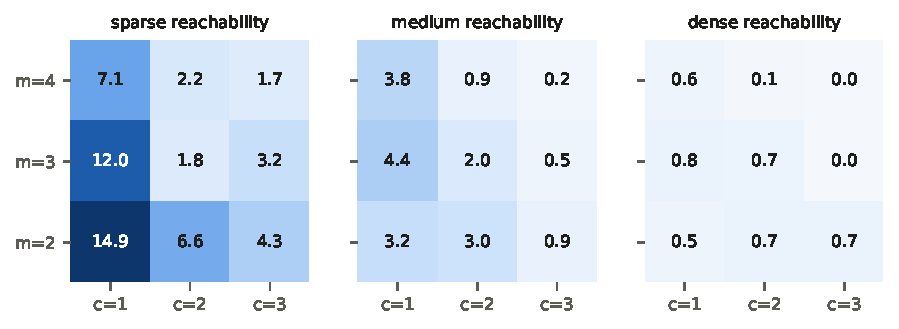
\includegraphics[width=0.92\textwidth]{fig_gain_heatmap.pdf}
\caption{Mean concealment gain $G(0)$ (\%) over 10 maps per cell, skewed priorities. Randomization pays only with sparse reachability and tight capacity ($c=1$), and the gain shrinks with more docks.}
\label{fig:heat}
\end{figure*}

\begin{figure}[!t]
\centering
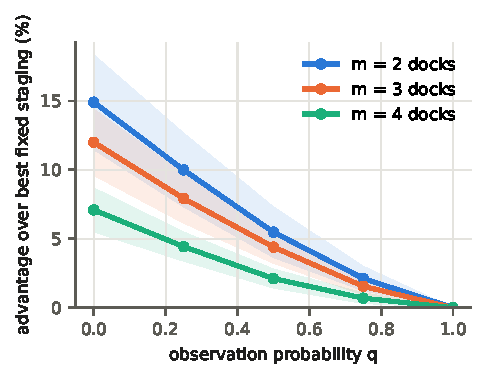
\includegraphics[width=0.9\columnwidth]{fig_q_curves.pdf}
\caption{Re-optimized advantage over the best fixed staging versus observation probability $q$ (sparse, skewed, $c=1$; mean $\pm$ s.e., 10 maps). Each instance's curve is convex and reaches zero at its own threshold $q^\star$. The plotted mean of piecewise-linear curves is itself convex but is not the curve of any single instance, and it reaches zero only at $q=1$ because $q^\star$ varies across maps; per-instance thresholds are summarized in the text.}
\label{fig:q}
\end{figure}


\subsection{Scaling to large facilities}
\textbf{Setup.} We generated larger instances on the same three map types with $K=20$ staging sites and $N\in\{30,40,50\}$ zones, using $m=3$ docks (1140 configurations), $n=6$ alarms, $c\in\{1,2\}$, sparse reachability and skewed priorities, with three layouts per map (54 instances). The attack spaces have $1.6\times10^6$ to $2.9\times10^7$ allocations and are never enumerated. Each instance is solved exactly with the matrix-free method for $q=0,0.25,0.5$.

\textbf{Results.} Table~\ref{tab:scale} reports the gains. The concealment benefit persists at facility scale. With $c=1$, every one of the 27 instances has a positive gain ($5$--$8\%$ on average at $q=0$). With $c=2$ the gain falls to about $2\%$, the same capacity effect as in Fig.~\ref{fig:heat}. Solving all three $q$ values took a median of $0.1$--$0.3$\,s per instance (maximum $0.62$\,s), with 1.3k--2.0k branch-and-bound nodes and, on average, fewer than 20 generated attacks per instance. Stress tests show where effort grows. With uniform priorities, which prune less, $N=30$ and $N=50$ took 9.1\,s and 5.7\,s ($4$--$7\times10^5$ nodes). With skewed priorities, $N=100$ zones, $K=30$ sites, $m=4$, $n=8$ and $c=2$ (27{,}405 configurations, $3.3\times10^{11}$ allocations) solved exactly for $q\in\{0,0.5\}$ in 11.5\,s.

\begin{table}[!t]
\centering
\caption{Matrix-free exact solutions on 30--50-zone maps (9 instances per row; mean $\pm$ 95\% CI). Time is the per-instance median of the total for all three $q$, including initialization and every exact pure worst case $\mu_d$ needed for $P$ and the LP rows, excluding Python start-up and one-time numba compilation. Maximum times and branch-and-bound statistics are in Supplementary Table~S2.}
\label{tab:scale}
\footnotesize\setlength{\tabcolsep}{3.5pt}
\begin{tabular}{@{}rrrrrrr@{}}
\toprule
$N$ & $|\W|$ & $c$ & $G(0)$ (\%) & $G(0.25)$ (\%) & $G(0.5)$ (\%) & time (s)\\
\midrule
30 & $1.6\mathrm{e}6$ & 1 & $7.8\pm2.7$ & $5.3\pm2.1$ & $3.0\pm1.6$ & 0.28\\
30 & $1.6\mathrm{e}6$ & 2 & $2.0\pm1.1$ & $1.2\pm0.7$ & $0.5\pm0.4$ & 0.13\\
40 & $8.2\mathrm{e}6$ & 1 & $5.0\pm2.2$ & $3.4\pm1.7$ & $2.0\pm1.2$ & 0.12\\
40 & $8.2\mathrm{e}6$ & 2 & $1.6\pm0.5$ & $1.0\pm0.4$ & $0.4\pm0.3$ & 0.11\\
50 & $2.9\mathrm{e}7$ & 1 & $5.2\pm1.6$ & $3.5\pm1.2$ & $1.9\pm0.7$ & 0.17\\
50 & $2.9\mathrm{e}7$ & 2 & $1.7\pm0.7$ & $0.9\pm0.5$ & $0.4\pm0.3$ & 0.13\\
\bottomrule
\end{tabular}
\end{table}


\subsection{Sensitivity analyses}\label{sec:sens}
\textbf{Policy-dependent relocation exposure.} We evaluated the end-to-end value of Remark~\ref{rem:reloc} on the 15 sparse layouts for shift lengths $H$ from 8\,h down to 2\,min. The exposure-aware policy is the best of the exogenous optima $x^\star(q')$, $q'\in[0,1]$, evaluated exactly under endogenous exposure. Relocation exposure $\mathbb{E}_x[\tau]/H$ of the exogenous optimum at $q=0$ is $0.1\%$, $0.9\%$, $3.7\%$, $11\%$ and $28\%$ for $H=8$\,h, 1\,h, 15\,min, 5\,min and 2\,min. The end-to-end gain at $q=0$ falls from $11.2\%$ to $10.6\%$ at 15\,min and $6.4\%$ at 2\,min, and exposure-aware re-optimization recovers at most 1.1 points (2\,min). The exogenous optimum stays above the best fixed configuration in at least 13 of 15 layouts at every $H$ and $q$, and the mean end-to-end threshold moves from $0.83$ to $0.79$. In closed loop with 15-minute shifts at $q=0.25$, the exogenous and exposure-aware policies gained $5.6\pm2.4\%$ and $5.3\pm2.4\%$ over fixed staging (13/15 layouts each), statistically indistinguishable. The exogenous-leakage optimum is therefore adequate for shifts of 15\,min or longer, while minute-scale re-staging requires modelling exposure explicitly (Supplementary Table~S3).

\textbf{Response model.} We re-solved the 240 grid games with $m\in\{3,4\}$ and $c\in\{1,2\}$ under three alternatives. In the favourable cell (sparse, $c=1$, skewed; 20 games), $G(0)$ is $9.5\pm3.0\%$ for the paper's all-or-nothing model with $p=0.7$, but $2.8\pm0.9\%$ with $p=0.5$, $15.4\pm4.9\%$ with $p=0.9$, and only $2.1\pm0.7\%$ under partial credit, where a zone earns $v_j$ times its fraction of resolved alarms. For partial credit the terminal problem is a transversal-matroid weighting solved exactly by a greedy rule, which matched an LP on 400 random cases. Per-instance gains under the two restoration rules correlate only at $r=0.48$. All-or-nothing restoration is what makes coordinated coverage valuable, so we restrict our conclusions to that model and to reliable robots; partial-credit or low-reliability settings must be re-solved before randomizing (Supplementary Table~S4).

\textbf{Scenario factors.} Table~\ref{tab:sens} varies one factor at a time around the simulation's base regime on the same 15 layouts, using the matrix-free solver. The gain grows with the alarm budget and priority skew, and shrinks with denser reachability, uniform priorities and a larger fleet. In the least favourable levels (uniform priorities, density $0.45$, $n=4$) it falls to 3--4\% and appears in only 7--11 of 15 layouts.

\begin{table}[!t]
\centering
\caption{One-factor-at-a-time sensitivity on the 15 map layouts (base$^\ast$: $m=3$, $c=1$, $n=6$, density $0.20$, Zipf priority exponent $\alpha=1$). Gains in \%, mean $\pm$ 95\% CI over layouts; $q^\star$ by bisection on the exact $V^\star(q)$.}
\label{tab:sens}
\footnotesize\setlength{\tabcolsep}{3.5pt}
\begin{tabular}{@{}llrrrr@{}}
\toprule
factor & level & $G(0)$ & $G(0.5)$ & $\bar q^\star$ & gain$>$0\\
\midrule
alarms $n$ & 4 & $3.7\pm2.0$ & $1.0\pm0.8$ & 0.44 & 10/15\\
alarms $n$ & 6$^\ast$ & $11.2\pm2.8$ & $4.2\pm1.7$ & 0.83 & 15/15\\
alarms $n$ & 8 & $14.6\pm3.9$ & $5.5\pm2.0$ & 0.89 & 15/15\\
density & 0.15 & $11.5\pm3.0$ & $4.2\pm1.6$ & 0.83 & 15/15\\
density & 0.2$^\ast$ & $11.2\pm2.8$ & $4.2\pm1.7$ & 0.83 & 15/15\\
density & 0.3 & $8.3\pm3.1$ & $3.1\pm1.5$ & 0.85 & 14/15\\
density & 0.45 & $3.6\pm2.0$ & $1.2\pm0.8$ & 0.57 & 11/15\\
priority skew $\alpha$ & 0.0 & $3.7\pm2.3$ & $1.8\pm1.2$ & 0.42 & 7/15\\
priority skew $\alpha$ & 0.5 & $5.3\pm1.2$ & $1.4\pm0.6$ & 0.77 & 15/15\\
priority skew $\alpha$ & 1.0$^\ast$ & $11.2\pm2.8$ & $4.2\pm1.7$ & 0.83 & 15/15\\
priority skew $\alpha$ & 2.0 & $28.3\pm12.6$ & $12.6\pm6.6$ & 0.79 & 14/15\\
$(m,c)$ & (3,1)$^\ast$ & $11.2\pm2.8$ & $4.2\pm1.7$ & 0.83 & 15/15\\
$(m,c)$ & (3,2) & $3.9\pm1.6$ & $0.6\pm0.4$ & 0.58 & 13/15\\
$(m,c)$ & (4,1) & $5.1\pm2.1$ & $1.4\pm0.7$ & 0.61 & 12/15\\
\bottomrule
\end{tabular}
\end{table}

\subsection{Closed-loop simulation}
\textbf{Setup.} We built three $120\times80$\,m occupancy-grid maps (Fig.~\ref{fig:maps}): a warehouse with shelf rows, an office with rooms and doors, and a campus with buildings. Each map has five random layouts of 12 staging sites and 12 zones. Robots move at a nominal 1.5\,m/s along 8-connected shortest paths, with a lognormal per-trip speed factor ($\sigma=0.15$) and a 30\,s service time. The deadline is set so that reachability density is $0.20$ (sparse regime, chosen from the passing cell $m=3$, $c=1$, skewed) or $0.60$ (dense control). A zone that no site reaches within the deadline is assigned its nearest site, with that arc's nominal travel time as its own deadline. Every shift lasts 8\,h. The policy draws a configuration, and docks are matched to the previous shift's docks so that robots relocate along shortest paths. An attack occurs at a uniform time; the attacker sees the realized staging if robots are still in transit or, independently, with probability $q$. The planner computes the optimal response under the nominal model. Each robot then drives from its actual position, mid-relocation if needed, and a request counts only if the robot arrives within the deadline and succeeds. We compare five policies: the best fixed configuration; an MEXCLP-style fixed placement; uniform randomization over all configurations; the concealed optimum $x^0$; and the leakage-aware optimum for the true $q$. Each (layout, policy, $q$) is run for 1000 shifts. Policies are compared with common random numbers: for a given (layout, $q$) every policy uses the same per-shift uniforms for the configuration draw, attack time and surveillance, and the same per-robot-slot speed and success draws, so differences are paired. The layout is the independent unit: we average the 1000 shifts within each layout and report 95\% $t$-intervals over the 15 layouts.

\begin{figure*}[!t]
\centering
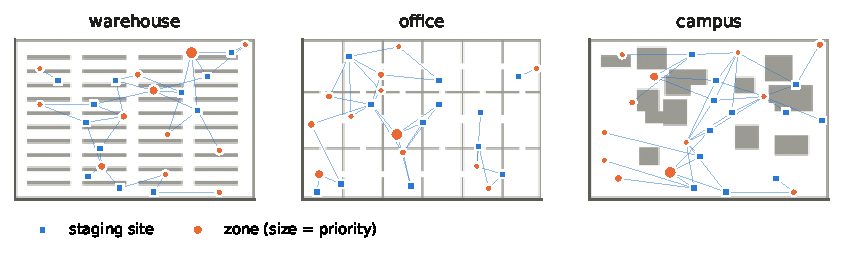
\includegraphics[width=0.92\textwidth]{fig_maps.pdf}
\caption{Simulation maps (layout 0). Lines mark site--zone pairs reachable within the deadline along obstacle-aware shortest paths (sparse regime).}
\label{fig:maps}
\end{figure*}

\textbf{Results.} Fig.~\ref{fig:sim} summarizes the 450 runs; every policy, regime and $q$ is tabulated in Supplementary Table~S1. In the sparse regime the leakage-aware policy improves on the best fixed staging by $8.1\pm2.7\%$ (15/15 layouts), $5.8\pm2.3\%$ (13/15) and $2.6\pm2.1\%$ (10/15) at $q=0,0.25,0.5$. At $q=0.5$ the unadapted concealed policy keeps only $0.9\pm2.4\%$ (7/15), so re-optimizing for leakage is what preserves the benefit. It also relocates robots less: 49\,m versus 71\,m per shift, because the optimal support shrinks as $q$ grows. Uniform randomization is consistently harmful ($-12$ to $-18\%$), since it spends probability on configurations with large gaps. Randomization helps only when the distribution is optimized. The MEXCLP placement was within $1\%$ of the fixed maximin. In the dense control regime the optimized and covering policies were statistically indistinguishable from fixed staging, as Fig.~\ref{fig:heat} predicts, while uniform randomization was still significantly worse ($-3.5\%$ to $-5.6\%$). Relocation took about 30\,s per shift, so in-transit exposure added only about $0.1\%$ to the observed fraction (Remark~\ref{rem:reloc}). Across all runs, simulated values correlate with the model value $V_x(q)$ at $r=0.955$ (Supplementary Fig.~S1). The simulator is on average 3.1\% lower than the model, because speed variation and mid-relocation positions cause deadline misses that the model omits.

\begin{figure*}[!t]
\centering
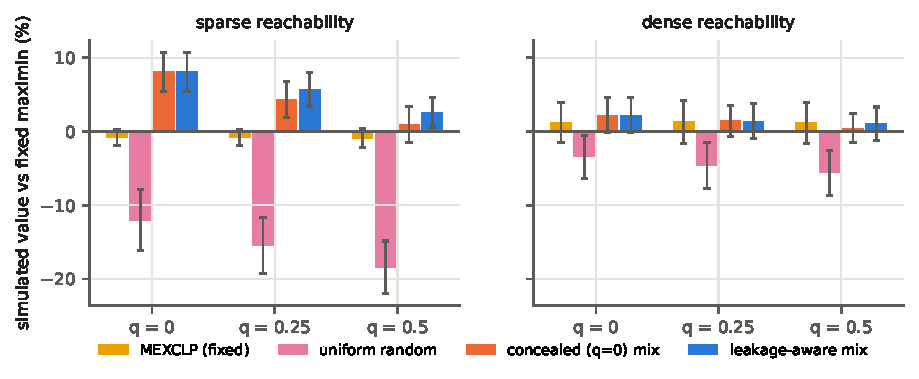
\includegraphics[width=0.92\textwidth]{fig_sim_bars.pdf}
\caption{Closed-loop simulation: mean change in restored value relative to the best fixed staging (95\% CI over 15 layouts across three maps; 1000 shifts each).}
\label{fig:sim}
\end{figure*}

\begin{figure*}[!t]
\centering
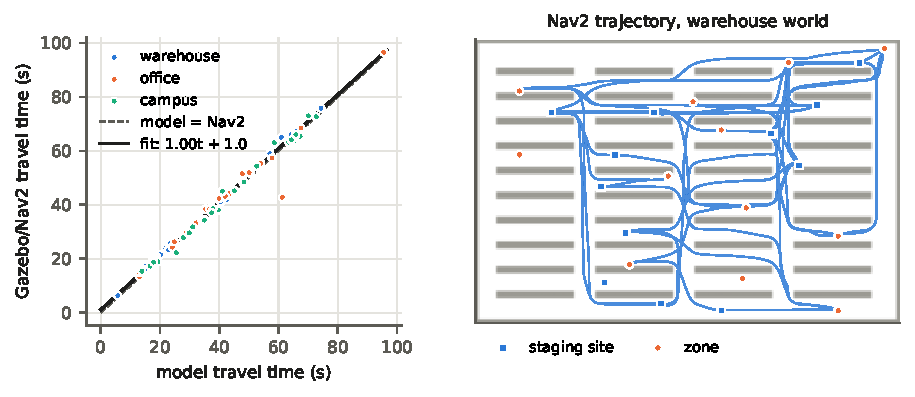
\includegraphics[width=0.92\textwidth]{fig_gazebo.pdf}
\caption{Gazebo/Nav2 validation. Left: measured Nav2 travel time against the model's grid travel time for 92 site--zone legs on three worlds (fit $0.997t+1.0$\,s, $R^2=0.995$). Right: the recorded Nav2 trajectory of the 40-leg warehouse tour.}
\label{fig:gz}
\end{figure*}






\subsection{Gazebo/Nav2: travel times, reachability and concurrent dispatch}
\textbf{Setup.} The model's reachability depends entirely on travel times from the grid path model, so we checked them against a full navigation stack. Each map's layout~0 was extruded into a Gazebo Harmonic world (1\,m walls). A Jackal-scale differential-drive robot ran ROS~2 Jazzy Nav2 on the static map at 0.25\,m resolution, with an A$^\ast$ NavFn planner, a Regulated Pure Pursuit controller at a desired 1.5\,m/s with curvature- and proximity-based slowdown, ground-truth odometry and default recovery behaviours. On each map the robot drove a 40-leg tour through randomly chosen sites and zones, so each leg measures one site--zone pair; every fifth leg was a site--site relocation. Travel time is measured in simulation time from goal acceptance to arrival within 0.5\,m.

\textbf{Results.} Of 120 legs, 118 succeeded. One failed from a software acknowledgement timeout under CPU load, and one from a controller stall near a building after the recovery behaviours were exhausted; we excluded each failure and the leg after it. Across the 92 response legs, Nav2 time $=0.997\,t_{\mathrm{model}}+1.0$\,s with $R^2=0.995$ (Fig.~\ref{fig:gz}). The uncalibrated mean absolute error is 3.7\%, and Nav2's mean effective speed is 1.45\,m/s against the nominal 1.5\,m/s. The largest deviation is conservative: Nav2 found a route 34\% shorter through a doorway that the 1\,m grid cannot traverse diagonally. With the paper's deadlines, the model and Nav2 classify 91 of the 92 measured pairs identically as reachable or not. Relocation legs took a median 1.03$\times$ the model time. We then rebuilt reachability for all 15 sparse layouts from the Nav2-calibrated times. The arcs agree with the model's on 98.7\% of pairs, and the re-optimized gain is $10.7\pm3.0\%$, $7.2\pm2.3\%$ and $4.0\pm1.7\%$ at $q=0,0.25,0.5$ (model: $11.2$, $7.5$, $4.2\%$), with mean $q^\star=0.82$ (model $0.83$). Policies designed on the grid model and evaluated on Nav2-calibrated reachability keep a gain in 13 of 15 layouts at every $q$ ($9.8\pm5.3\%$ at $q=0$). Near the deadline the agreement is equally tight. On the 37 legs within 10\,s of their deadline, the median absolute error was 0.9\,s, and the 95th-percentile error over all legs was 3.8\,s. With every deadline tightened by that 3.8\,s, the re-optimized gain is still $10.8\%$, $7.2\%$ and $3.9\%$ at $q=0,0.25,0.5$. These single-robot results validate the travel-time and reachability model only.

\textbf{Concurrent multi-robot dispatch.} To test the full response under concurrency, we ran three robots at once in Gazebo, each with its own namespaced Nav2 stack and TF tree (same configuration; robots do not perceive each other, as costmaps use the static map), on the representative warehouse layout~1 and office layout~0. Each layout received 3 fixed-staging shifts and 20 shifts drawn from the leakage-aware policy at $q=0.25$, with paired success draws. In each shift the robots were placed at the drawn docks, the attack was drawn as in the simulator, and all dispatch goals were sent simultaneously. Over 46 shifts and 53 dispatched legs (23 shifts with two or three robots moving at once), successful legs arrived $0.95$\,s (8\%) later than the model on average, and concurrency caused no failure (per-shift results in Supplementary Tables~S6--S9). Robots sent to the same zone point did converge to within 0.48\,m, so deployments need distinct service points per alarm. Two deterministic model--navigation discrepancies did appear. A forced arc whose deadline equals its nominal time (zero slack) was missed by 1.0--1.3\,s in all 6 of its uses, and one office arc ending near a wall made the Regulated Pure Pursuit collision check stall in all 10 of its uses. The leakage-aware policy's realized value exceeded fixed staging by $6.5\%$ on the warehouse layout (model with the same draws: $11.4\%$), and by $0.0\%$ on the office layout (model: $10.3\%$): one unverified arc erased the entire benefit. We therefore re-planned with \emph{Nav2-verified reachability}, dropping arcs whose slack is below the 3.8\,s error bound and arcs Nav2 failed to complete. The model gains become $2.6\%$ and $10.2\%$, and in Gazebo the realized gains over fixed staging were $3.4\%$ and $15.8\%$, with all 18 dispatched legs on time and the realized value equal to the model's (same draws) in every shift; the 20-shift samples happen to exceed the expected gains. Verification also lowers the attainable value itself (best fixed value $13.5\to11.0$ and $14.6\to12.7$), since the unverified model had overstated what the robots can reach. Every verified shift dispatches a single robot, so these runs used one Nav2 stack. With three full stacks on our two-core machine, the planner intermittently failed to acknowledge goals within the behaviour tree's timeout (5 of 18 legs), an infrastructure limit of the test machine that we report in Supplementary Tables~S10--S11. Reachability should therefore be verified with the deployed navigation stack before policies are computed. These experiments cover up to three robots without inter-robot perception; they do not exercise congestion at scale or robot--robot avoidance.



\section{Discussion and Limitations}
The results support a narrow but actionable conclusion. Randomized staging is worth deploying when reachability is sparse, dock capacity is tight and the probability that the realized staging leaks is clearly below $q^\star$. Because $q^\star$ and its certified lower bound vary widely between maps (Fig.~\ref{fig:q}), they should be computed per site rather than assumed. The study has limits. Alarm budgets are small ($n\le8$), and branch-and-bound effort grows when priorities are uniform, because value ordering then prunes less. The conclusions are restricted to all-or-nothing restoration with independent, reasonably reliable robots: partial credit or $p=0.5$ cuts the favourable-cell gain to about 2--3\% (Sec.~\ref{sec:sens}), and correlated failures or heterogeneous robots would change \eqref{eq:U} and the bounds built on it. The policies are optimal for exogenous leakage; they remain adequate for shifts of 15\,min or longer, but minute-scale re-staging needs exposure-aware optimization. The adversary is fully rational and knows the policy. The model omits navigation failures, and the concurrent Gazebo runs show that one unverified arc can erase the benefit, so reachability must be verified with the deployed stack. Those runs involve at most three robots without inter-robot perception, there is no hardware experiment, and the maps are synthetic. Testing on real facility maps and robots is the next step.

\section{Conclusion}
We formulated leakage-aware randomized staging for capacity-constrained multi-robot response. We showed that the decision must be made over joint configurations rather than marginals, characterized the observation threshold $q^\star$ beyond which randomization loses its strict worst-case advantage, and computed it exactly with one LP. Pre-specified experiments, closed-loop simulation, sensitivity analyses and Gazebo/Nav2 runs agree on where randomization pays and where it does not, and show that optimizing it for the expected leakage, on verified reachability, matters as much as randomizing at all. Code, instances, the pre-specified protocol and all raw results are released at~\cite{alam2026code}.

\small
\begin{thebibliography}{99}
\bibitem{tambe2011} M. Tambe, \emph{Security and Game Theory: Algorithms, Deployed Systems, Lessons Learned}. Cambridge Univ. Press, 2011.
\bibitem{korzhyk2011} D. Korzhyk, Z. Yin, C. Kiekintveld, V. Conitzer, and M. Tambe, ``Stackelberg vs. Nash in security games: An extended investigation of interchangeability, equivalence, and uniqueness,'' \emph{J. Artif. Intell. Res.}, vol. 41, pp. 297--327, 2011.
\bibitem{agmon2008} N. Agmon, S. Kraus, and G. A. Kaminka, ``Multi-robot perimeter patrol in adversarial settings,'' in \emph{Proc. IEEE ICRA}, 2008.
\bibitem{basilico2012} N. Basilico, N. Gatti, and F. Amigoni, ``Patrolling security games: Definition and algorithms for solving large instances with single patroller and single intruder,'' \emph{Artif. Intell.}, vol. 184--185, pp. 78--123, 2012.
\bibitem{kiekintveld2009} C. Kiekintveld, M. Jain, J. Tsai, J. Pita, F. Ord\'o\~nez, and M. Tambe, ``Computing optimal randomized resource allocations for massive security games,'' in \emph{Proc. AAMAS}, 2009.
\bibitem{mcmahan2003} H. B. McMahan, G. J. Gordon, and A. Blum, ``Planning in the presence of cost functions controlled by an adversary,'' in \emph{Proc. ICML}, 2003.
\bibitem{jain2011} M. Jain, D. Korzhyk, O. Van\v{e}k, V. Conitzer, M. P\v{e}chou\v{c}ek, and M. Tambe, ``A double oracle algorithm for zero-sum security games on graphs,'' in \emph{Proc. AAMAS}, 2011.
\bibitem{xu2015leak} H. Xu, A. X. Jiang, A. Sinha, Z. Rabinovich, S. Dughmi, and M. Tambe, ``Security games with information leakage: Modeling and computation,'' in \emph{Proc. IJCAI}, 2015.
\bibitem{xu2015asym} H. Xu, Z. Rabinovich, S. Dughmi, and M. Tambe, ``Exploring information asymmetry in two-stage security games,'' in \emph{Proc. AAAI}, 2015.
\bibitem{han2016} C. Y. Han, B. J. Lunday, and M. J. Robbins, ``A game theoretic model for the optimal location of integrated air defense system missile batteries,'' \emph{INFORMS J. Comput.}, 2016, doi:10.1287/ijoc.2016.0690.
\bibitem{boardman2017} N. T. Boardman, B. J. Lunday, and M. J. Robbins, ``Heterogeneous surface-to-air missile defense battery location: A game theoretic approach,'' \emph{J. Heuristics}, vol. 23, pp. 417--447, 2017.
\bibitem{brown2006} G. Brown, M. Carlyle, J. Salmer\'on, and K. Wood, ``Defending critical infrastructure,'' \emph{Interfaces}, vol. 36, no. 6, pp. 530--544, 2006.
\bibitem{delage2019} E. Delage, D. Kuhn, and W. Wiesemann, ```Dice'-sion-making under uncertainty: When can a random decision reduce risk?'' \emph{Manage. Sci.}, vol. 65, no. 7, pp. 3282--3301, 2019.
\bibitem{church1974} R. Church and C. ReVelle, ``The maximal covering location problem,'' \emph{Pap. Reg. Sci. Assoc.}, vol. 32, pp. 101--118, 1974.
\bibitem{daskin1983} M. S. Daskin, ``A maximum expected covering location model: Formulation, properties and heuristic solution,'' \emph{Transp. Sci.}, vol. 17, no. 1, pp. 48--70, 1983.
\bibitem{gerkey2004} B. P. Gerkey and M. J. Matari\'c, ``A formal analysis and taxonomy of task allocation in multi-robot systems,'' \emph{Int. J. Robot. Res.}, vol. 23, no. 9, pp. 939--954, 2004.
\bibitem{gale1957} D. Gale, ``A theorem on flows in networks,'' \emph{Pacific J. Math.}, vol. 7, no. 2, pp. 1073--1082, 1957.
\bibitem{charnes1962} A. Charnes and W. W. Cooper, ``Programming with linear fractional functionals,'' \emph{Nav. Res. Logist. Q.}, vol. 9, no. 3--4, pp. 181--186, 1962.
\bibitem{alam2026code} S. M. Alam and H. Rafique, ``Code and data for leakage-aware robot staging,'' 2026. [Online]. Available: https://github.com/alam121/hub-placement
\end{thebibliography}
\end{document}
